\PassOptionsToPackage{dvipsnames}{color}
\documentclass[10pt]{NSP1}
\usepackage{url,floatflt,cite}
\usepackage{helvet,times}
\usepackage{psfig,graphicx}
\usepackage{mathptmx,amsmath,amssymb,bm}
\usepackage{float}
\usepackage[bf,hypcap]{caption}
\usepackage{placeins}
\usepackage{booktabs}
\usepackage{array}
\usepackage{multirow}
\usepackage{makecell}
\usepackage{subcaption}

\tolerance=1
\emergencystretch=\maxdimen
\hyphenpenalty=10000
\hbadness=10000
\topmargin=0.00cm
\addtolength{\oddsidemargin}{.5in}
\addtolength{\evensidemargin}{-.5in}

\def\sm{\smallskip}
\def\no{\noindent}

\def\firstpage{1}
\setcounter{page}{\firstpage}
\def\thevol{15}
\def\thenumber{1}
\def\theyear{2026}

% Float placement parameters to prevent figures/tables from being delayed to end
\renewcommand{\topfraction}{0.95}
\renewcommand{\bottomfraction}{0.95}
\renewcommand{\dbltopfraction}{0.95}
\renewcommand{\textfraction}{0.05}
\renewcommand{\floatpagefraction}{0.75}
\renewcommand{\dblfloatpagefraction}{0.75}

\makeatletter
\renewcommand\section{\@startsection{section}{1}{\z@}%
  {-8pt plus -2pt minus -1pt}%
  {4pt plus 1pt minus 1pt}%
  {\normalsize\bfseries}}
\renewcommand\subsection{\@startsection{subsection}{2}{\z@}%
  {-6pt plus -1.5pt minus -1pt}%
  {2.5pt plus 1pt minus 0.5pt}%
  {\normalsize\bfseries\itshape}}
\renewcommand\subsubsection{\@startsection{subsubsection}{3}{\z@}%
  {-4pt plus -1pt minus -0.5pt}%
  {1.5pt plus 0.5pt minus 0.5pt}%
  {\normalsize\itshape}}
\makeatother

\raggedbottom
\setlength{\parskip}{0pt}
\setlength{\intextsep}{6pt plus 2pt minus 1pt}
\setlength{\textfloatsep}{8pt plus 2pt minus 1pt}
\setlength{\floatsep}{6pt plus 2pt minus 1pt}
\setlength{\abovecaptionskip}{4pt plus 1pt minus 1pt}
\setlength{\belowcaptionskip}{4pt plus 1pt minus 1pt}

\begin{document}

\titlefigurecaption{\large \bf \rm \vspace{0.15cm}International Journal of Thin Films Science and Technology}

\title{\textbf{Structural and Spectroscopic Investigation of Bismuth Oxide Thin Films}}

\author{Karamvir Tanwar$^{1}$ and David Joseph$^{1,*}$}

\institute{
$^1$Department of Physics, Guru Jambheshwar University of Science \& Technology, Hisar-125001, Haryana, India
}

\titlerunning{Structural and Spectroscopic Investigation of Bismuth Oxide Thin Films}
\authorrunning{K. Tanwar and D. Joseph}

%corresponding author email
\mail{davidjoseph@gjust.org}

\received{-- ---. 2026}
\revised{-- ---. 2026}
\accepted{-- ---. 2026}
\published{-- ---. 2026}

\abstracttext{Bismuth oxide (Bi$_2$O$_3$) thin films were synthesized on glass substrates via the thermal evaporation technique at ambient room temperature, followed by a post-deposition air-annealing treatment at 500~$^\circ$C for 2 hours. The structural, morphological, vibrational, and surface chemical states of the film matrices were systematically investigated to uncover the underlying physical mechanisms of thermal restructuring. X-ray diffraction (XRD) analysis revealed that the post-treated films were polycrystalline, exhibiting a pure monoclinic $\alpha$-Bi$_2$O$_3$ crystal structure with a preferred growth orientation along the $(\bar{1}21)$ lattice plane. Field emission scanning electron microscopy (FESEM) examinations demonstrated a well-developed, granular microstructure with distinct crystallite boundaries and an interconnected porous geometry. Energy dispersive X-ray spectroscopy (EDAX) confirmed the high chemical purity of the films, mapping a uniform distribution of Bismuth and Oxygen matching the expected stoichiometry. Laser Raman spectra and FTIR displayed sharp, prominent vibrational modes characteristic of long-range lattice framework order, tracking a slight increase in transmittance and peak sharpening driven by thermal dehydration. A high-resolution XPS confirmed the complete elimination of sub-oxides, where positive shifts in the core-level binding energies of the resolved Bi4f$_{7/2}$ and Bi4f$_{5/2}$ spin-orbit doublets verified the stabilization of the pure Bi$^{3+}$ chemical valence state.}

\keywords{Bismuth Oxide, Thermal Evaporation, Optical properties, XRD, Laser Raman Spectra, FE-SEM, EDAX, FTIR, XPS.}

\maketitle

\section{Introduction}

Bismuth oxide (Bi$_2$O$_3$) thin films represent a class of highly functional materials that are of great scientific interest. Especially for solid-state applications such as optoelectronic coatings, transparent ceramic glasses, microwave-integrated circuits, and contemporary energy storage systems, where polymorphic metal oxide architectures exist. The material's intrinsic physical characteristics, such as its wide optical energy gap (ranging from 2.0 to 3.96~eV), notable dielectric permittivity, and prominent photoconductive properties, are fundamental to its broad technological relevance \cite{R1,R2}. The low-temperature monoclinic $\alpha$-phase, the tetragonal $\beta$-phase, the body-centered cubic $\gamma$-phase, and the high-temperature face-centered cubic $\delta$-phase are the four main distinct polymorphic modifications into which Bi$_2$O$_3$ crystallizes. The exact stabilization of a desired phase is a crucial goal for advanced device engineering because each of these structural configurations displays noticeably distinct lattice parameters, bonding symmetries, and physical responses \cite{R3,R4}.

The choice of synthesis procedures and processing environments greatly affects the surface chemical states, localized vibrational modes, and specific structural arrangement in thin-film forms. Because of its cost-effectiveness, high deposition rates, ease of parameter control, and capacity to produce extremely dense coatings with excellent substrate adhesion, physical vapour deposition via thermal evaporation continues to be the industry standard for large-scale operations \cite{R5}. The fast thermal quenching of vaporized species onto room-temperature substrates, however, usually produces highly disordered, amorphous, or chemically non-stoichiometric as-deposited networks beset by localized oxygen deficiencies or metastable phases. This is a recurring problem in vacuum thermal evaporation \cite{R6,R7}. In order to provide the thermal activation energy required to overcome kinetic barriers, promote atomic diffusion, and initiate structural restructuring toward long-range crystalline order, post-deposition thermal annealing is widely used \cite{R8,R9}. A comprehensive understanding of the localized structural, vibrational, and chemical state evolution during the transition from the as-deposited disordered state to a thermally annealed crystalline matrix at 500~$^\circ$C is still lacking despite numerous studies into the general properties of bismuth oxide \cite{R10,R11}. Further physical mechanisms controlling lattice macrostrain relaxation, functional group configurations, and the precise valence stability of the Bismuth ion (Bi$^{3+}$) post-thermal processing are frequently ignored in many previous reports that only concentrate on macroscopic optical parameters. Mapping the direct correlation between atomic-level modifications (healing of oxygen vacancies and vibrational symmetry restoration) and macroscopic physical restructuring (grain growth and pore elimination) is a clear research gap \cite{R12,R13}.

In order to fill this knowledge gap, the current work methodically examines the structural, morphological, vibrational, and chemical characteristics of thin films made by vacuum thermal evaporation on glass substrates, which are then subjected to a controlled ambient post-deposition annealing process at 500~$^\circ$C for two hours. We specifically monitor the phase transformation pathways, surface restructuring dynamics, and chemical state modifications using an integrated, complementary characterisation suite that includes X-ray Diffraction (XRD), Field Emission Scanning Electron Microscopy integrated with Energy Dispersive X-ray Spectroscopy (FESEM/EDAX), Raman scattering, Fourier Transform Infrared spectroscopy (FTIR), and X-ray Photoelectron Spectroscopy (XPS). For high-performance thin-film device integrations, the insights gained from this thorough cross-property analysis offer a solid foundation for optimising the processing-structure relationships of evaporated bismuth oxide film networks.

\section{Materials and Methods}

Bismuth oxide Bi$_2$O$_3$ thin films were synthesized on commercially available glass substrates operating a vacuum thermal evaporation system. High-purity Bi$_2$O$_3$ powder (99.9\% purity, melting point $\sim$817~$^\circ$C) was employed as the precursor charge source and loaded into a specialized molybdenum boat. Before deposition, the glass substrates underwent a rigorous multi-step ultrasonic cleaning routine consisting of sequential baths in acetone, ethanol, and deionized water, followed by drying under a filtered hot-air stream to eliminate surface contaminants. Inside the evaporation chamber, the vertical working distance separating the molybdenum boat and the cleaned glass substrates was rigidly fixed at 10~cm. The chamber was evacuated to a reliable base pressure of $5\times10^{-5}$~mbar before initiating thermal vaporization. At room temperature, the as-deposited thin-film matrices were found to have a nominal thickness of about 0.5~$\mu$m. Post-deposition annealing profiles were carried out in an ambient atmospheric furnace at 500~$^\circ$C for a continuous duration of 2~h under a controlled heating rate, followed by natural cooling to room temperature in order to examine thermal restructuring patterns.

X-ray diffraction (XRD) was used to assess the crystallographic structure, phase evolution, and lattice parameters of both the as-deposited and thermally treated films using a Rigaku SmartLab system 3kW running with Cu-K$\alpha$ radiation ($\lambda = 1.5406$~\AA). An attached EDAX module was used for elemental tracking and stoichiometric validation, while Field Emission Scanning Electron Microscopy (FESEM; JEOL JSM-7610F Plus) was used to record surface microstructural morphology, grain boundaries, and cross-sectional features. Using FTIR and a laser Raman spectrometer, the short-range molecular arrangements and localized vibrational profiles were cross-examined. Additionally, XPS was used to examine the constituent species' electronic binding energy distributions, core-level oxidation configurations, and surface chemical states.

\begin{figure}[H]
\centering
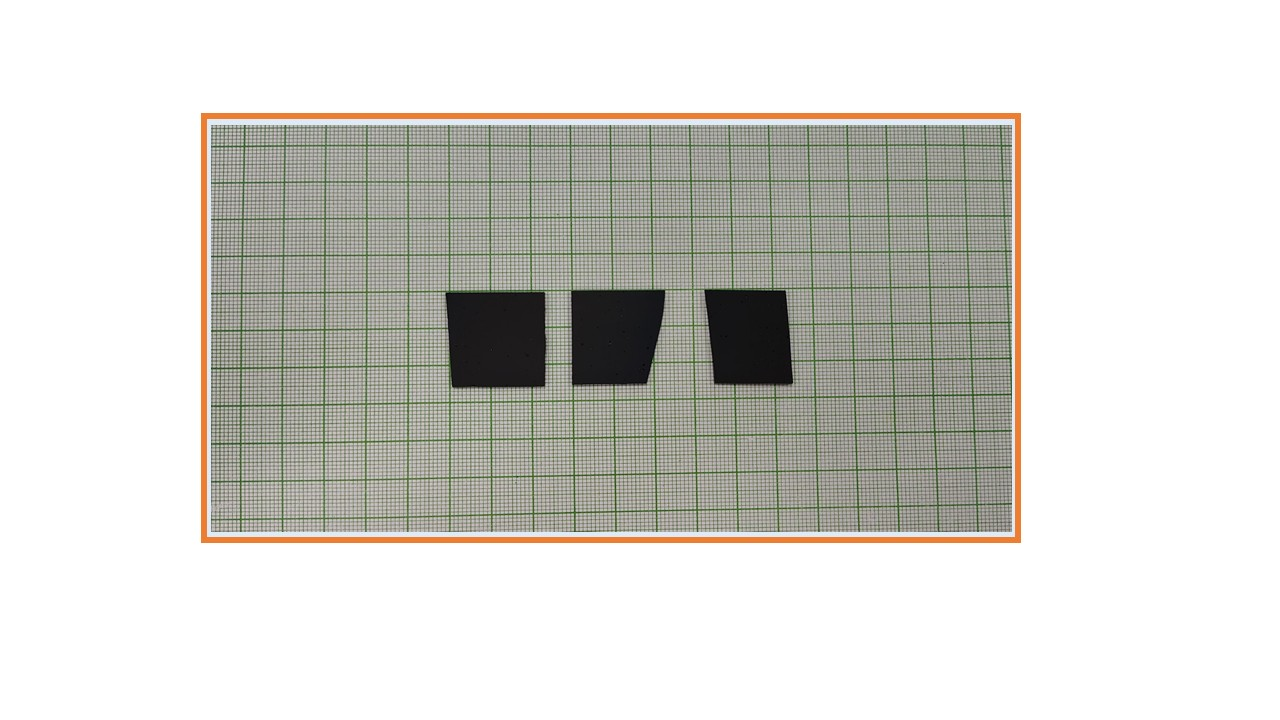
\includegraphics[width=0.88\linewidth]{media/fig1.jpeg}
\caption{Photograph of the Bi$_2$O$_3$ thin films synthesized via thermal evaporation.}
\label{fig1}
\end{figure}

\section{Results and Discussions}

\subsection{X-ray Diffraction (XRD) Analysis}

The phase structure, crystallographic orientation, and phase transformation dynamics of the bismuth oxide thin films were evaluated using X-ray diffraction over a wide $2\theta$ scanning range of 20$^\circ$--80$^\circ$. Figure~\ref{fig2} illustrates the highly crystalline diffraction pattern recorded from the sample subjected to thermal annealing at 500~$^\circ$C for 2~h. The post-deposition annealing process causes a major transformation profile, whereas as-deposited thermally evaporated films usually exhibit a disordered or amorphous structure because of the quick thermal quenching of vaporized species arriving at an unheated substrate. Furthermore, the ($hkl$) values agreed well with the standard JCPDS card values, which indicated a monoclinic structure \cite{R15}.

\begin{figure}[H]
\centering
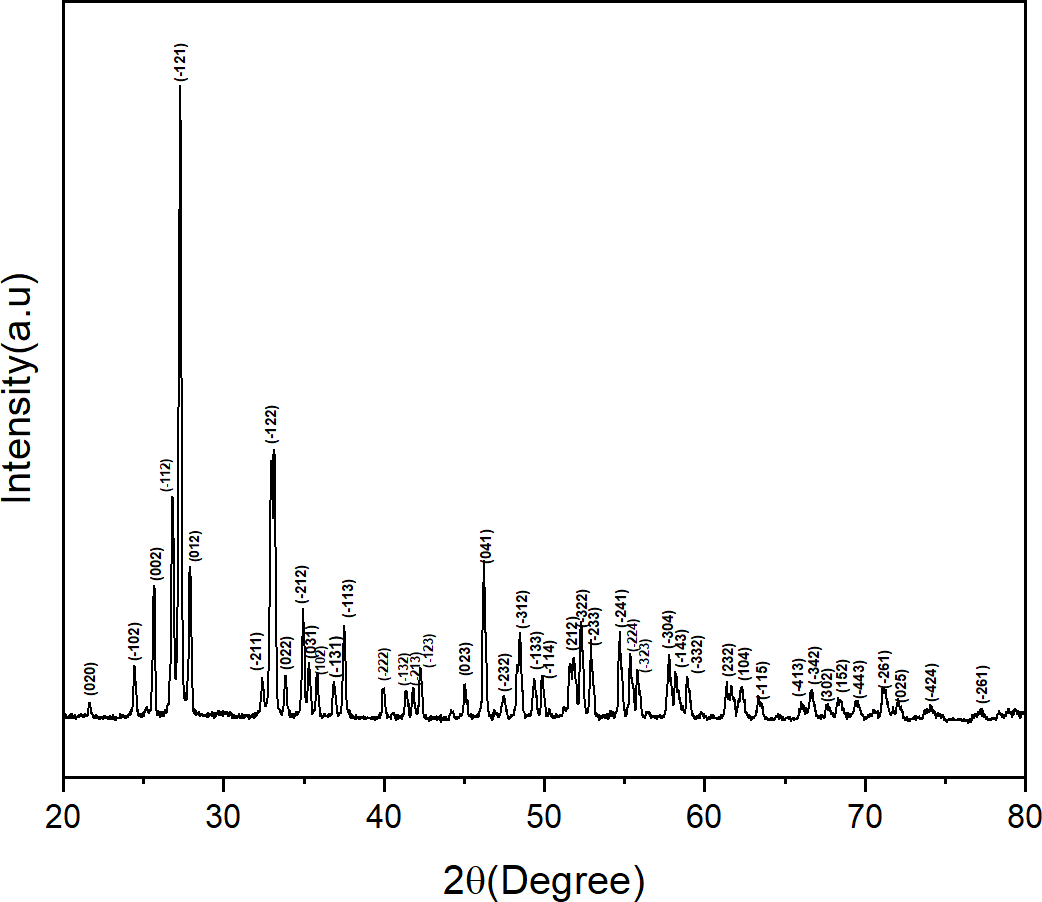
\includegraphics[width=0.98\linewidth]{media/fig2.png}
\caption{XRD pattern of the Bi$_2$O$_3$ thin film on a glass substrate after subsequent annealing treatment at 500~$^\circ$C for 2~h.}
\label{fig2}
\end{figure}

Every single reflection peak indexed in Figure~\ref{fig2} aligns with the standard reference values of the pure monoclinic $\alpha$-phase of bismuth oxide ($\alpha$-Bi$_2$O$_3$), agreeing with standard data metrics. The high-density $(\bar{1}21)$ lattice plane is assigned to the strong, dominant reflection at $2\theta \approx 27.33^\circ$, indicating a preferred texturing effect along this particular orientation during crystallization. Further distinctive reflections at $2\theta \approx 25.68^\circ$, $26.91^\circ$, $28.02^\circ$, $33.24^\circ$, and $46.28^\circ$ are smoothly assigned to the monoclinic cells $(002)$, $(\bar{1}12)$, $(012)$, $(\bar{1}22)$, and $(041)$ atomic planes, respectively. Within the measurement limits, no secondary peaks corresponding to residual metallic bismuth (Bi) or other polymorphs (tetragonal $\beta$, cubic $\gamma$, or cubic $\delta$) are found, indicating high phase purity.

The experimental Interplanar spacing ($d$-spacing) values determined by Bragg's Law ($\lambda = 2d \sin\theta$) were methodically modelled against the theoretical framework for a monoclinic system in order to assess the unit cell metrics \cite{R16,R17}. The basic connection between the lattice dimensions, Miller indices ($hkl$), and Interplanar spacing is described as:
\begin{equation}
\frac{1}{d^2} = \frac{1}{\sin^2\beta} \left\{ \frac{h^2}{a^2} + \frac{k^2 \sin^2\beta}{b^2} + \frac{l^2}{c^2} - \frac{2hl\cos\beta}{ac} \right\} \label{eq1}
\end{equation}
where lattice parameters are $a = 5.8444$, $b = 8.1574$, $c = 7.5032$ and $\beta = 112.97^\circ$.

Table~\ref{tab1} describes the full matching between the theoretically predicted values using Equation~(\ref{eq1}) and the experimental $d$-spacing entries.

\begin{table*}[t]
\centering
\caption{Interplanar spacing and Miller indices.}
\label{tab1}
\setlength{\tabcolsep}{4.5pt}
\footnotesize
\begin{tabular}{ccccc|c|ccccc}
\toprule
\textbf{Sr. No.} & \textbf{2$\theta$ ($^\circ$)} & \textbf{Observed $d$} & \textbf{Standard $d$} & \textbf{Plane ($hkl$)} & \quad & \textbf{Sr. No.} & \textbf{2$\theta$ ($^\circ$)} & \textbf{Observed $d$} & \textbf{Standard $d$} & \textbf{Plane ($hkl$)} \\
\midrule
1.  & 21.71 & 4.090 & 4.083 & (020)          & & 24. & 49.92 & 1.825 & 1.823 & ($\bar{1}$14) \\
2.  & 24.00 & 3.627 & 3.622 & ($\bar{1}$02)  & & 25. & 51.71 & 1.767 & 1.765 & (212)         \\
3.  & 25.68 & 3.461 & 3.456 & (002)          & & 26. & 52.34 & 1.746 & 1.745 & ($\bar{3}$22) \\
4.  & 26.91 & 3.313 & 3.311 & ($\bar{1}$12)  & & 27. & 52.92 & 1.727 & 1.725 & ($\bar{2}$33) \\
5.  & 27.33 & 3.258 & 3.253 & ($\bar{1}$21)  & & 28. & 54.66 & 1.675 & 1.673 & ($\bar{2}$41) \\
6.  & 28.02 & 3.187 & 3.182 & (012)          & & 29. & 55.36 & 1.657 & 1.655 & ($\bar{2}$24) \\
7.  & 32.42 & 2.754 & 2.753 & ($\bar{2}$11)  & & 30. & 55.86 & 1.644 & 1.642 & ($\bar{3}$23) \\
8.  & 32.89 & 2.800 & 2.709 & ($\bar{1}$22)  & & 31. & 57.80 & 1.596 & 1.594 & ($\bar{3}$04) \\
9.  & 33.01 & 2.640 & 2.638 & (022)          & & 32. & 58.16 & 1.583 & 1.581 & ($\bar{1}$43) \\
10. & 33.24 & 2.560 & 2.558 & ($\bar{1}$12)  & & 33. & 58.92 & 1.575 & 1.574 & ($\bar{3}$32) \\
11. & 35.40 & 2.535 & 2.532 & (031)          & & 34. & 61.38 & 1.509 & 1.506 & (232)         \\
12. & 35.91 & 2.500 & 2.498 & (102)          & & 35. & 62.42 & 1.488 & 1.485 & (104)         \\
13. & 36.95 & 2.431 & 2.429 & ($\bar{1}$31)  & & 36. & 63.34 & 1.466 & 1.462 & ($\bar{1}$15) \\
14. & 37.51 & 2.391 & 2.389 & ($\bar{1}$13)  & & 37. & 66.04 & 1.412 & 1.408 & ($\bar{4}$13) \\
15. & 39.94 & 2.251 & 2.249 & ($\bar{2}$22)  & & 38. & 66.66 & 1.402 & 1.401 & ($\bar{3}$42) \\
16. & 41.42 & 2.177 & 2.175 & ($\bar{1}$32)  & & 39. & 67.60 & 1.384 & 1.383 & (302)         \\
17. & 41.87 & 2.155 & 2.154 & ($\bar{2}$13)  & & 40. & 68.31 & 1.368 & 1.367 & (152)         \\
18. & 42.34 & 2.133 & 2.131 & ($\bar{1}$23)  & & 41. & 69.56 & 1.351 & 1.348 & ($\bar{4}$43) \\
19. & 45.12 & 2.008 & 2.006 & (023)          & & 42. & 71.22 & 1.323 & 1.319 & ($\bar{1}$61) \\
20. & 46.28 & 1.960 & 1.957 & (041)          & & 43. & 72.08 & 1.309 & 1.309 & (025)         \\
21. & 47.42 & 1.918 & 1.915 & ($\bar{2}$32)  & & 44. & 74.64 & 1.279 & 1.279 & ($\bar{4}$24) \\
22. & 48.44 & 1.875 & 1.879 & ($\bar{3}$12)  & & 45. & 77.24 & 1.234 & 1.233 & ($\bar{2}$61) \\
23. & 49.38 & 1.843 & 1.840 & ($\bar{1}$33)  & &     &       &       &       &               \\
\bottomrule
\end{tabular}
\end{table*}

Thermal activation energy dynamics influence the underlying physical mechanism, which results in the observed peak sharpening (the significant narrowing of the Full Width at Half Maximum, or FWHM) and high relative intensities. Long-range atomic diffusion is made possible by the atoms absorbing sufficient thermal energy to break unstable local bonds within the amorphous vapor-quenched film cluster during ambient air annealing at 500~$^\circ$C. A large-scale crystallization into the monoclinic structure results from the constituent bismuth and oxygen ions migrating into their optimal thermodynamic coordination positions due to this thermal drive. At the same time, internal structural defects are healed, grain boundaries are sharply minimized through coalescence, and structural micro-strain in the thin-film configuration is significantly reduced as a result of this atomic reorganization. The pattern's high, well-resolved Bragg reflections are the result of an enhanced crystallite configuration brought about by the severe lattice strain relaxation.

\subsection{Laser Raman Spectra}

Laser Raman spectroscopy (WITEC alpha 3000Ri) at room temperature was used to cross-examine short-range molecular symmetries and localized vibrational properties in order to supplement the bulk crystallographic insights obtained from X-ray diffraction. The Raman scattering spectrum of the 500~$^\circ$C annealed bismuth oxide thin film network recorded under a 532~nm excitation source over a wavenumber shift window up to 2500~cm$^{-1}$ is shown in Figure~\ref{fig3}.

\begin{figure}[H]
\centering
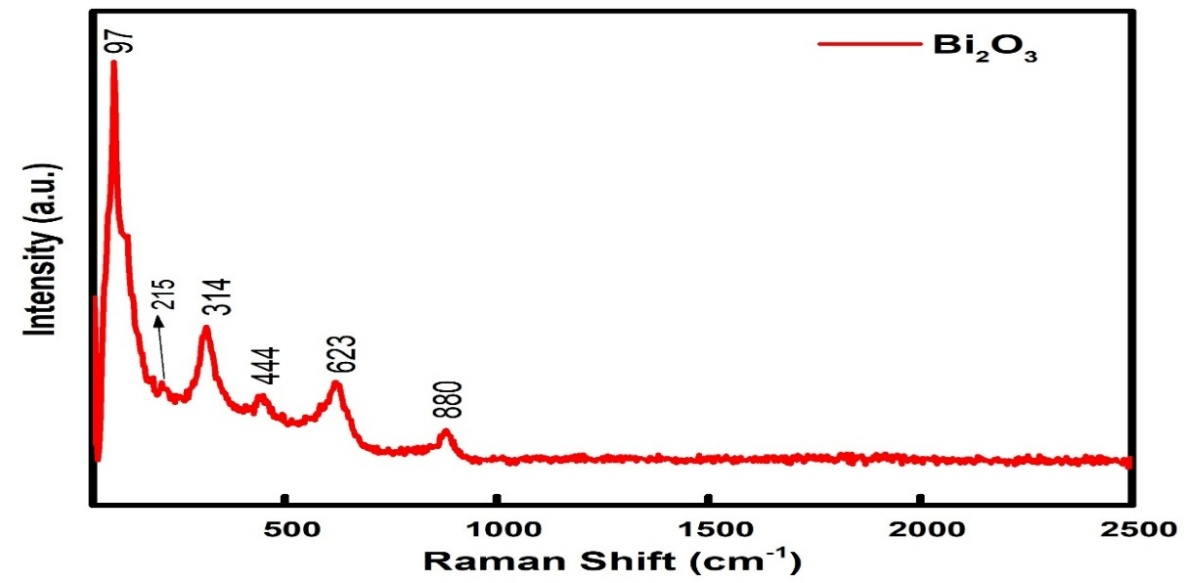
\includegraphics[width=0.98\linewidth]{media/fig3.jpeg}
\caption{Raman Spectrum of the Bi$_2$O$_3$ thin film recorded at an excitation wavelength of 532~nm.}
\label{fig3}
\end{figure}

According to factor group theoretical predictions, the monoclinic $\alpha$-Bi$_2$O$_3$ lattice architecture (space group $P2_1/c$) indicates that sixty foundational lattice modes are obtained from the total irreducible vibrational representation. Of these, precisely thirty optical phonon components are distributed through symmetry of ($\Gamma_{\text{Raman}} = 15A_g + 15B_g$) and are categorised as strictly Raman-active modes \cite{R18}. A clear structural fingerprint confirming the pure monoclinic phase was observed in the recorded spectrum, which displayed distinct, well-resolved scattering peaks at 97, 215, 314, 444, 623, and 880~cm$^{-1}$. The external translation dynamics of heavy (Bi$^{3+}$) cations in the unit cell framework essentially controlled the extremely strong, sharp low-frequency mode that appeared at 97~cm$^{-1}$. The internal structural bending configurations and stretching modes connected to the specialized Bi--O bonds in the polyhedral networks were responsible for the intermediate-energy peaks located at 215, 314, and 444~cm$^{-1}$. The localized stretching dynamics of terminal Bi--O bonds within the oxygen-coordinated polyhedra were represented by the high-energy features that appeared at 623~cm$^{-1}$ and 880~cm$^{-1}$ \cite{R19,R20}.

\subsection{FESEM Analysis}

A field-emission scanning electron microscope (FESEM) was used at different configurations to examine the surface morphological characteristics and architectural cross-sections of both the as-deposited and post-deposition heat-treated bismuth oxide thin films. The explicit morphological changes that took place throughout the thin film matrix are shown in Figures~\ref{fig4}a to \ref{fig4}d. The as-deposited vacuum-evaporated thin film matrix first showed a highly disordered, uniform, and fine particulate distribution, as shown in Figure~\ref{fig4}a. This arrangement is typical of physical vapour deposition on substrate materials at room temperature, where incoming vaporised clusters experience fast thermal quenching, limiting lateral atomic mobility on the surface. A notable restructuring profile occurred after the film was exposed to a high thermal annealing threshold of 500~$^\circ$C for two hours in air (Figure~\ref{fig4}b). In line with the strong Bragg reflections observed by X-ray diffraction, the film underwent a transition into a clearly defined, continuous granular architecture with sharp grain clusters, suggesting significantly improved crystallinity.

According to high-magnification surface monitoring at 75,000$\times$ (Figure~\ref{fig4}c), the annealed film had an average grain size of roughly 34 $\pm$ 3~nm. Similar cross-sectional analysis at the same high-resolution view fields (Figure~\ref{fig4}d) revealed a network of interconnected pores in the thin-film structure with an average pore size of 36 $\pm$ 6~nm.

Grain boundary migration and coalescence dynamics driven by thermal activation energy. The atoms in the thin-film network absorbed enough thermal energy to propel long-range surface and volume diffusion processes when it was annealed at 500~$^\circ$C. In order to reduce the overall excess surface free energy linked to disordered grain boundary interfaces, smaller, metastable grains merged or coalesced into nearby clusters. Localised lattice defects were gradually eliminated as larger grain configurations grew via this coalescence mechanism, resulting in the film's clean crystallisation into the monoclinic structure \cite{R21,R22}. The observed uniform microporous geometry throughout the bulk matrix was simultaneously created by the spatial distribution of escaping trapped gases, residual solvent traces, or structural volume shrinkage during the phase crystallisation process, stabilising the thin-film infrastructure's physical boundaries.

\begin{figure*}[t]
\centering
\begin{subfigure}[b]{0.45\textwidth}
  \centering
  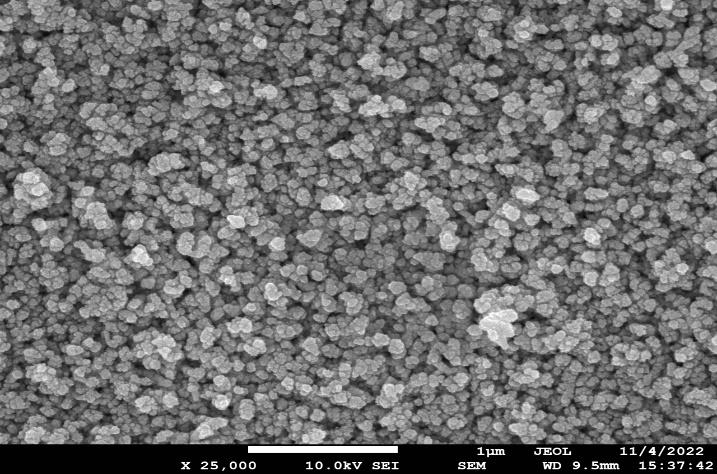
\includegraphics[width=\linewidth,height=5.2cm,keepaspectratio]{media/fig4a.png}
  \caption{}
  \label{fig4a}
\end{subfigure}\hfil
\begin{subfigure}[b]{0.45\textwidth}
  \centering
  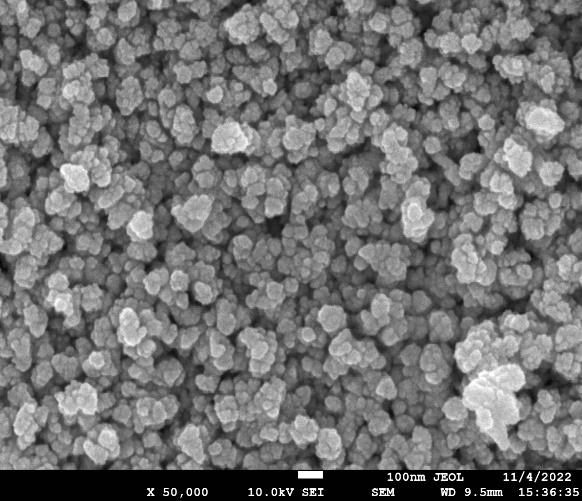
\includegraphics[width=\linewidth,height=5.2cm,keepaspectratio]{media/fig4b.png}
  \caption{}
  \label{fig4b}
\end{subfigure}
\vskip 4pt
\begin{subfigure}[b]{0.45\textwidth}
  \centering
  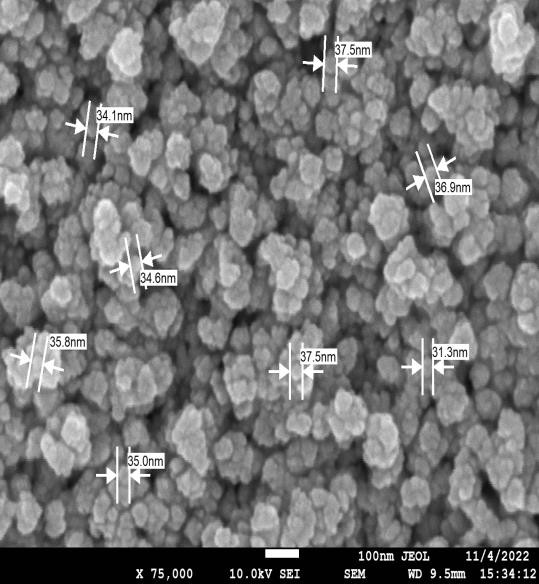
\includegraphics[width=\linewidth,height=5.2cm,keepaspectratio]{media/fig4c.jpeg}
  \caption{}
  \label{fig4c}
\end{subfigure}\hfil
\begin{subfigure}[b]{0.45\textwidth}
  \centering
  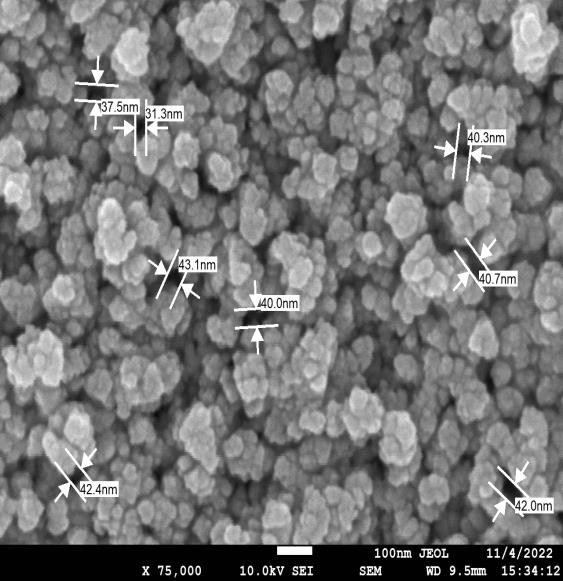
\includegraphics[width=\linewidth,height=5.2cm,keepaspectratio]{media/fig4d.jpeg}
  \caption{}
  \label{fig4d}
\end{subfigure}
\caption{FESEM images of the Bi$_2$O$_3$ thin films: (a) surface micrograph of the as-deposited film captured at 25,000$\times$ magnification, (b) surface morphology after thermal annealing at 500~$^\circ$C captured at 50,000$\times$ magnification, (c) high-resolution surface topology at 75,000$\times$ magnification confirming an average grain size of 34 $\pm$ 3~nm, and (d) cross-sectional microstructure at 75,000$\times$ magnification revealing an average internal pore size distribution of 36 $\pm$ 6~nm.}
\label{fig4}
\end{figure*}

\subsection{EDAX Analysis}

Energy dispersive X-ray spectroscopy (EDAX) analysis was used to determine the elemental composition, chemical purity, and stoichiometric distributions within the synthesised bismuth oxide thin film networks. The representative EDAX spectrum obtained from the thin film matrix after thermal annealing at approximately 500~$^\circ$C is shown in Figure~\ref{fig5}.

\begin{figure}[H]
\centering
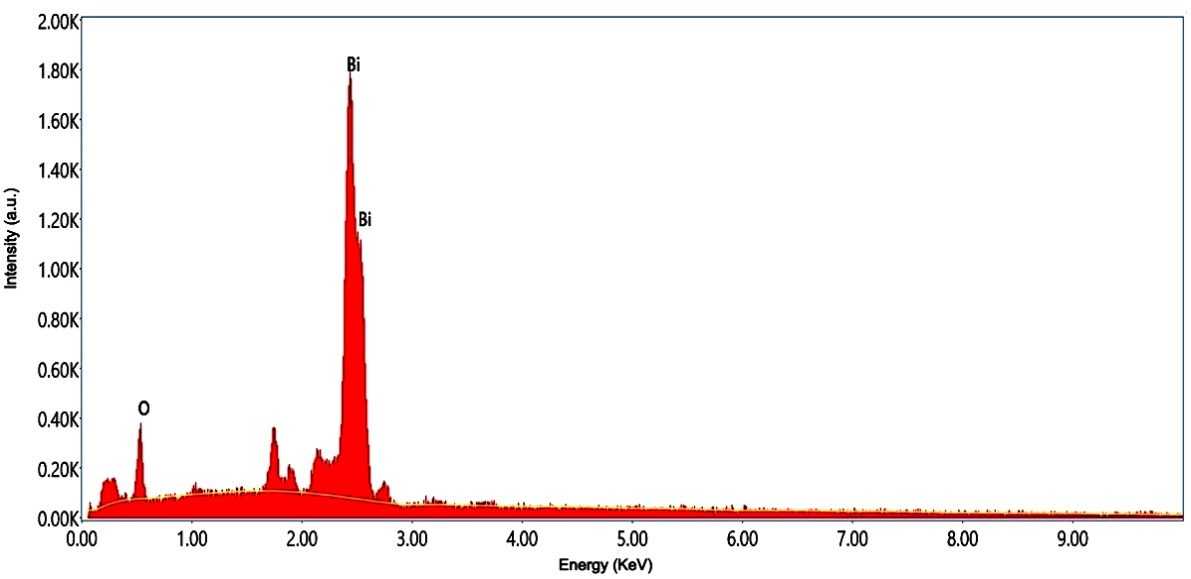
\includegraphics[width=0.98\linewidth]{media/fig5.jpeg}
\caption{Prominent EDAX peaks corresponding to bismuth and oxygen.}
\label{fig5}
\end{figure}

The spectrum clearly showed distinctive, well-resolved X-ray emission peaks that exclusively corresponded to the core shells of bismuth (Bi) and oxygen (O). The electronic transitions corresponding to the Bi-M series shell were found to be the extremely intense emission lines clustered between 2.3~keV and 2.6~keV. Simultaneously, the distinct peak that emerged at a lower energy threshold of about 0.52~keV was clearly attributed to the typical O-K$\alpha$ radiation profile. The underlying glass substrate matrix was the source of minor background features that appeared close to the lower energy spectrum limit \cite{R23}. Beyond these anticipated components, the total lack of any secondary or unexpected foreign emission lines throughout the assessed energy range attested to the high chemical purity of the produced thin films and confirmed that there was no cross-contamination during the vacuum thermal evaporation or subsequent open-air thermal annealing processes.

The ambient thermal oxidation dynamics that are active during the post-deposition annealing process are the fundamental physical mechanism that controls the observed elemental distribution. Due to the different vapour pressures and dissociation rates of bismuth and oxygen species under high vacuum, physical vapour deposition via vacuum thermal evaporation often results in non-stoichiometric matrices with significant sub-oxides or localized oxygen deficiencies in their as-deposited state. The absorbed thermal energy triggered long-range oxygen diffusion from the surrounding atmosphere directly into the porous thin-film networks when the thin film was exposed to a high thermal threshold of 500~$^\circ$C in an outdoor setting. The oxygen ions were able to fill empty lattice centers and form direct bonds with sub-stoichiometric bismuth clusters thanks to this high-temperature atmospheric interaction. Consequently, this reaction driven by thermal diffusion successfully optimized the elemental balance, shifting the overall system toward the ideal 2:3 atomic ratios necessary to stabilize the pure, stable monoclinic $\alpha$-Bi$_2$O$_3$ matrix structure confirmed by the prior XRD and Raman profiles \cite{R24}. Table~\ref{tab2} compiles the localized quantitative elemental atomic percentages and weight variations taken from this EDAX baseline.

\begin{table}[H]
\centering
\caption{Elemental Composition of the Bi$_2$O$_3$ thin film sample.}
\label{tab2}
\setlength{\tabcolsep}{4pt}
\small
\begin{tabular}{cccc}
\toprule
\textbf{Sr. No.} & \textbf{Elements} & \makecell{\textbf{Expected}\\\textbf{Atomic \%}} & \makecell{\textbf{Observed}\\\textbf{Atomic \%}} \\
\midrule
1. & O  & 60 & 63.5 \\
2. & Bi & 40 & 33.5 \\
\bottomrule
\end{tabular}
\end{table}

\subsection{Fourier Transform Infrared Spectroscopy (FTIR) Analysis}

Fourier-transform infrared (FTIR) spectroscopy was employed to identify the functional groups, chemical bond configurations, and structural evolution of the bismuth oxide thin films before and after annealing processing. FTIR spectra were recorded over the wavenumber range of 4000--400~cm$^{-1}$ using a Perkin-Elmer spectrometer. The stretching modes of adsorbed hydroxyl (O--H) groups are responsible for the transmittance peaks at 3785.92~cm$^{-1}$ and 3552.18~cm$^{-1}$ for the as-deposited film \cite{R25}. These peaks shift to 3724.72~cm$^{-1}$ and 3532.72~cm$^{-1}$ after annealing at 500~$^\circ$C because of thermal dehydration. After thermal processing, the (C--H) asymmetric stretching vibration at 2925~cm$^{-1}$ in the as-deposited state splits into distinct symmetric and asymmetric doublets at 2920~cm$^{-1}$ and 2851~cm$^{-1}$, suggesting a structural reorganization of surface organic contaminants. Additionally, after annealing, a sharp structural framework peak at 1205~cm$^{-1}$ replaces the intense carbonate stretching band at 1458~cm$^{-1}$ in the as-deposited sample. A graphical representation of the FTIR spectral data for the as-deposited and annealed bismuth oxide thin films is presented in Figure~\ref{fig6}a and Figure~\ref{fig6}b \cite{R26,R27}.

\begin{figure*}[t]
\centering
\begin{subfigure}[b]{0.45\textwidth}
  \centering
  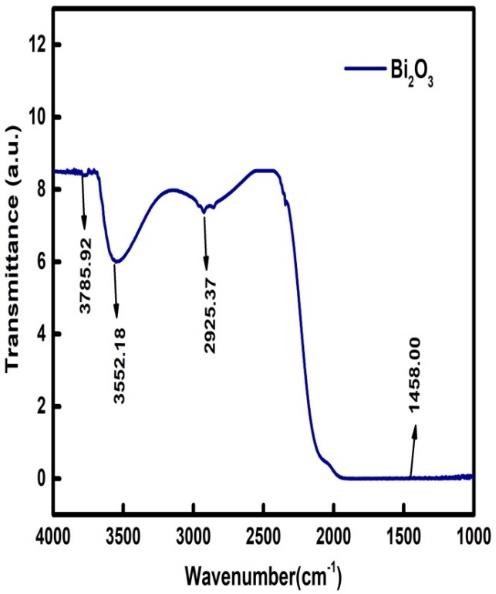
\includegraphics[width=\linewidth,height=5.0cm,keepaspectratio]{media/fig6a.jpeg}
  \caption{}
  \label{fig6a}
\end{subfigure}\hfil
\begin{subfigure}[b]{0.45\textwidth}
  \centering
  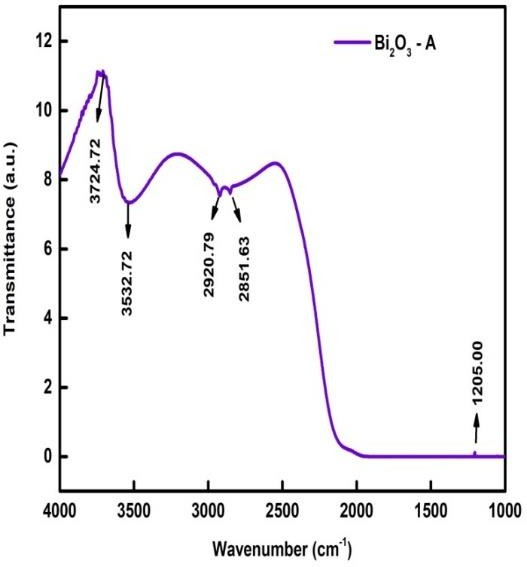
\includegraphics[width=\linewidth,height=5.0cm,keepaspectratio]{media/fig6b.jpeg}
  \caption{}
  \label{fig6b}
\end{subfigure}
\caption{Comparative FTIR transmittance spectra profiles of the synthesized bismuth oxide thin film matrices: (a) the as-deposited film network showcasing surface contaminant absorption modes, and (b) the post-deposition annealed film (500~$^\circ$C for 2~h) showing moisture elimination and the emergence of the crystalline $\alpha$-Bi$_2$O$_3$ structural matrix network.}
\label{fig6}
\end{figure*}

Significant, wide transmittance minima were found for the as-deposited thin film (Figure~\ref{fig6}a), with centers at 3785.92~cm$^{-1}$ and 3552.18~cm$^{-1}$. After the post-deposition annealing process at 500~$^\circ$C, these bands showed a discernible sharpening and shifted lower to 3724.72~cm$^{-1}$ and 3532.72~cm$^{-1}$ (Figure~\ref{fig6}b). At the same time, a weak hydrocarbon environmental trace signature (C--H) asymmetric stretch was found at 2925.37~cm$^{-1}$ in the as-deposited amorphous phase, separated into a clear, sharp doublet at 2920.79~cm$^{-1}$ and 2851.63~cm$^{-1}$ following thermal processing. In the lower wavenumber regime, the most significant structural variation was recorded. A characteristic surface contaminant carbonate stretching node at approximately 1458.00~cm$^{-1}$ was observed in the as-deposited profile, which showed a wide, deep absorption zone extending below 2000~cm$^{-1}$. The higher-order vibrational harmonics of the localised Bi--O--Bi bridging networks inside the monoclinic lattice unit cells are represented by a distinct, sharp framework signature that emerged at 1205.00~cm$^{-1}$ after thermal annealing at 500~$^\circ$C, completely suppressing the carbonate band. The surrounding bismuth and oxygen ions condensed into their corresponding coordination sites as these structural impurities disappeared. Because molecular disorder was eliminated, the material's localised damping effects were reduced, allowing for unrestricted lattice vibrations. Sharp peak shifts and the emergence of the unique monoclinic metal-oxygen framework signature at 1205.00~cm$^{-1}$ were caused by this structural optimisation, which directly supported the high structural order and phase purity observed in the XRD and Raman spectra.

Vibration band positions (wavenumbers) and corresponding transmittance percentages (T\%) for as-deposited and annealed (500~$^\circ$C, 2~h) Bi$_2$O$_3$ thin films are summarized in Table~\ref{tab3}.

\begin{table*}[t]
\centering
\caption{Comparison of FTIR transmission peaks for as-deposited and annealed Bi$_2$O$_3$ thin films.}
\label{tab3}
\resizebox{\textwidth}{!}{%
\begin{tabular}{clcccc}
\toprule
\textbf{Peak} & \textbf{Vibrational Assignment Mode} & \textbf{As-deposited Film (Bi$_2$O$_3$)} & \textbf{As-deposited Films} & \textbf{Annealed Film (Bi$_2$O$_3$)} & \textbf{Annealed Films} \\
\textbf{No.}  &                                      & \textbf{Wavenumber (cm$^{-1}$)}         & \textbf{Transmittance (T\%)} & \textbf{Wavenumber (cm$^{-1}$)}     & \textbf{Transmittance (T\%)} \\
\midrule
1 & O--H stretching Vibration (Adsorbed Moisture)     & 3785.92 & 8.38 & 3724.72 & 11.01 \\
2 & O--H stretching Vibration (Adsorbed Moisture)     & 3552.18 & 6.00 & 3532.33 & 7.33  \\
3 & C--H Symmetric stretching Vibration              & 2925.37 & 7.37 & 2920.79 & 7.54  \\
4 & Bi--O--Bi Monoclinic lattice structural framework & 1458.00 & 0.02 & 2851.63 & 7.61  \\
5 & ---                                              & ----    & ---- & 1205.00 & 0.00  \\
\bottomrule
\end{tabular}%
}
\end{table*}

\subsection{X-ray Photoelectron Spectroscopy (XPS) Analysis}

X-ray photoelectron spectroscopy (XPS) analysis was performed to confirm the localized core-level configurations, oxidation parameters, and surface chemical electronic states of the synthesised thin-film matrix. The high-resolution core-level XPS spectrum of the Bismuth (Bi4f) region for the thin film after post-deposition thermal treatment at approximately 500~$^\circ$C for two hours, recorded over a narrow binding energy window from 154~eV to 166~eV, is shown in Figure~\ref{fig7}.

\begin{figure}[H]
\centering
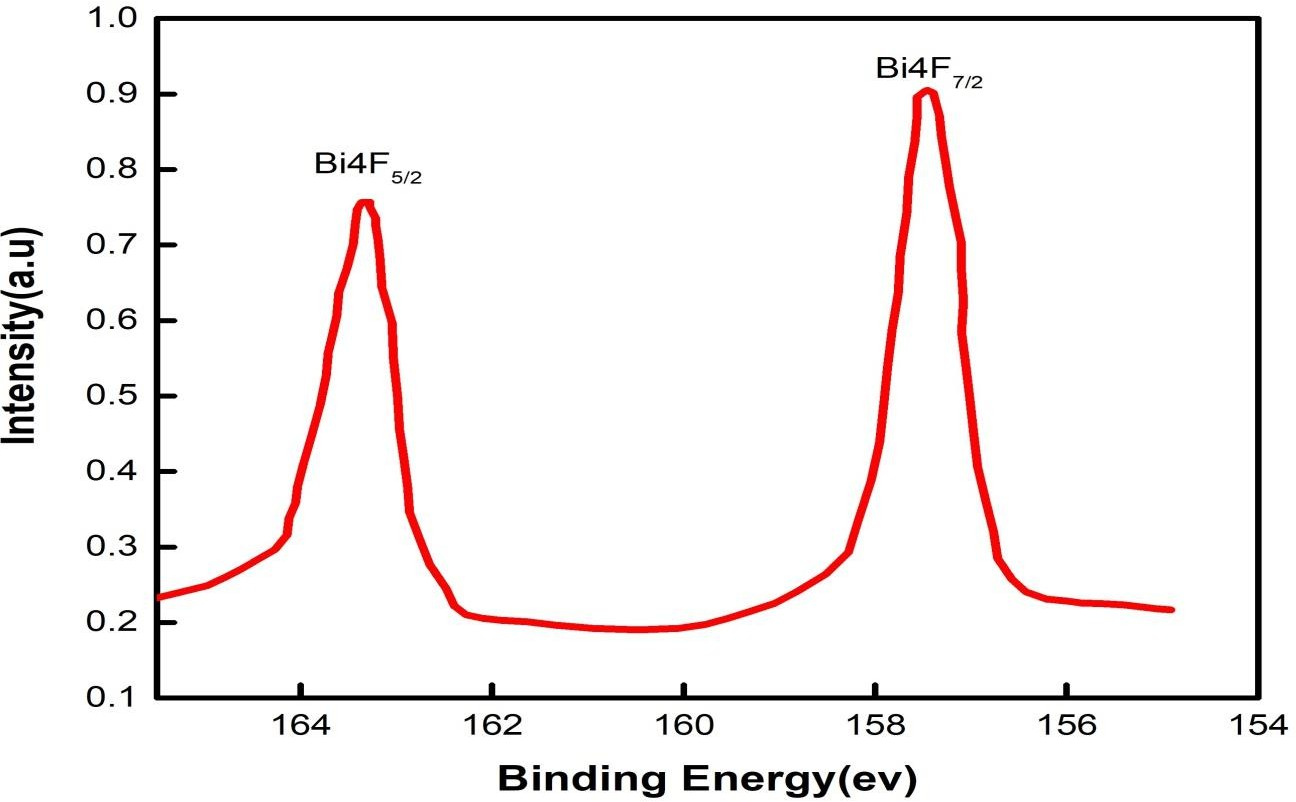
\includegraphics[width=0.98\linewidth]{media/fig7.jpeg}
\caption{XPS core-level spectrum of the Bi4f region for the Bi$_2$O$_3$ thin film annealed at 500~$^\circ$C on a glass substrate, displaying the resolved Bi4f$_{7/2}$ and Bi4f$_{5/2}$ spin-orbit doublets validating the stable (Bi$^{3+}$) oxidation state.}
\label{fig7}
\end{figure}

The high-resolution profile showed symmetric line shapes with negligible asymmetric tailing, resolving into a clear, sharp spin-orbit doublet core level. The distinctive spin-orbit split states were identified as the well-resolved peaks that appeared at binding energies of 163.32~eV and 157.42~eV, respectively. It was determined that the evaluated spin-orbit splitting energy separation ($\Delta E$) between these two doublet peaks is precisely 5.9~eV. Bismuth is stable in its nominal trivalent oxidation state (Bi$^{3+}$), which establishes the formation of a chemically pure bismuth oxide network. This is confirmed by both the absolute binding energy centers and this clean 5.9~eV splitting parameter.

Lattice stoichiometry restoration and oxygen vacancy annihilation directly control the underlying physical mechanism causing the observed binding energy shift after annealing. High-vacuum thermally evaporated thin-film matrices often have a sub-stoichiometric sub-oxide phase and a high density of localised oxygen vacancies (V$_{\text{O}}$). Because of these structural flaws, there is a localised build-up of excess electron density around nearby bismuth cations. This increases electrostatic shielding effects and causes the core-level binding energies to shift downward, closer to metallic Bi, which normally resides around 156.5~eV. When the thin film was exposed to a regulated thermal processing profile at 500~$^\circ$C in ambient atmospheric air, ambient oxygen atoms quickly permeated into the film matrix's microporous channels. The oxygen vacancies were effectively filled by this structural integration. The core-level binding energy of the Bi 4f$_{7/2}$ peak shifted upward toward its fully oxidised value as a result of the decreased localised electronic screening surrounding the Bismuth nuclei. The structural stability and elemental ratios monitored by XRD, Raman, and EDAX are confirmed by this positive binding energy shift, which fully validates the optimisation of the chemical state \cite{R28,R29}.

\section{Conclusion}

Single-phase monoclinic $\alpha$-Bi$_2$O$_3$ thin films were successfully grown on glass substrates using vacuum thermal evaporation followed by a systematic open-air thermal annealing process at 500~$^\circ$C for 2~h. X-ray diffraction and laser Raman scattering analyses cross-confirmed a complete structural transformation from a disordered as-deposited network into a highly crystalline, pure monoclinic phase with a preferred orientation along the $(\bar{1}21)$ lattice plane, which is strongly supported by the factor group summary model $\Gamma_{\text{Raman}} = 15A_g + 15B_g$.

FESEM micrographs tracked an annealing-induced morphological restructuring characterized by distinct grain expansion to an average size of 34 $\pm$ 3~nm and an interconnected porous framework with a mean feature diameter of 36 $\pm$ 6~nm, driven by grain boundary migration and surface free energy minimization. Functional FTIR transmissions and quantified EDAX elemental tracking demonstrated that thermal processing effectively removed carbonaceous trace residues and surface-adsorbed water, starting ambient oxygen diffusion to maintain internal stoichiometry.

Lastly, a positive binding energy shift in the resolved Bi4f$_{7/2}$ (157.42~eV) and Bi4f$_{5/2}$ (163.32~eV) doublets confirmed the stabilisation of the pure Bi$^{3+}$ oxidation state, and core-level XPS spectra verified the total removal of sub-oxides. These closely related structural and chemical results show how well vacuum evaporation and post-deposition thermal treatment work together to create high-quality, phase-pure Bi$_2$O$_3$ film matrices suitable for sophisticated solid-state and thin-film device integrations.

\section*{Acknowledgments}

The authors would like to thank TAS, New Delhi, for assistance with sample synthesis, and the Central Instrumentation Laboratory (CIL), Guru Jambheshwar University of Science \& Technology, Hisar, for sample characterization. One of the authors, Karamvir, is grateful to the Council of Scientific and Industrial Research (CSIR), New Delhi, for the award of a Junior Research Fellowship/Senior Research Fellowship (JRF/SRF).

\begin{thebibliography}{99}
\setlength{\itemsep}{0.8pt plus 0.2pt}
\setlength{\parskip}{0pt}

\bibitem{R1} L. Leontie, M. Caraman, M. Delibas, G. I. Rusu, Materials Research Bulletin \textbf{36}(9), 1629--1637 (2001).

\bibitem{R2} L. Leontie, G. I. Rusu, Journal of Non-Crystalline Solids \textbf{352}(9--20), 1475--1478 (2006).

\bibitem{R3} T. P. Gujar, V. R. Shinde, C. D. Lokhande, R. S. Mane, S. H. Han, Applied Surface Science \textbf{250}(1--4), 161--167 (2005).

\bibitem{R4} M. Fruth, D. Popa, R. Berger, M. Ramer, A. Gartner, M. Ciulei, M. Zaharescu, Journal of the European Ceramic Society \textbf{25}(12), 2171--2174 (2005).

\bibitem{R5} K. Brezesinski, R. Ostermann, P. Hartmann, J. Perlich, T. Brezesinski, Chemistry of Materials \textbf{22}(10), 3079--3085 (2010).

\bibitem{R6} T. N. Soitah, Y. Chunhui, Y. Yong, N. Yinghua, S. Liang, Current Applied Physics \textbf{10}(6), 1372--1377 (2010).

\bibitem{R7} J. C. Medina, M. Bizarro, P. Silva-Bermudez, M. Giorcelli, A. Tagliaferro, S. E. Rodil, Thin Solid Films \textbf{612}, 72--81 (2016).

\bibitem{R8} C. L. Gomez, O. Depablos-Rivera, J. C. Medina, P. Silva-Bermudez, S. Muhl, A. Zeinert, S. E. Rodil, Solid State Ionics \textbf{255}, 147--152 (2014).

\bibitem{R9} P. L. Popa, S. S{\o}nderby, S. Kerdsongpanya, J. Lu, H. Arwin, P. Eklund, Thin Solid Films \textbf{624}, 41--48 (2017).

\bibitem{R10} Z. Sun, D. Oka, T. Fukumura, Crystal Growth \& Design \textbf{19}(12), 7170--7174 (2019).

\bibitem{R11} P. H. Falsetti, F. C. Soares, G. N. Rodrigues, D. M. Del Duque, W. R. de Oliveira, B. F. Gianelli, V. R. de Mendonca, Materials Today Communications \textbf{27}, 102214 (2021).

\bibitem{R12} J. Sydorenko, M. Krunks, A. Katerski, R. Grzibovskis, A. Vembris, A. Mere, I. O. Acik, RSC Advances \textbf{14}(28), 19648--19657 (2024).

\bibitem{R13} I. Boudene, M. Oubakalla, M. El Bouji, M. Beraich, R. A. Belakhmima, A. Zarrouk, M. E. Belghiti, Surfaces and Interfaces \textbf{75}, 107808 (2025).

\bibitem{R14} A. Iljinas, L. Marcinauskas, Thin Solid Films \textbf{594}, 192--196 (2015).

\bibitem{R15} T. P. Gujar, V. R. Shinde, C. D. Lokhande, Materials Research Bulletin \textbf{41}(8), 1558--1564 (2006).

\bibitem{R16} G. Malmros, L. Fernholt, C. J. Ballhausen, U. Ragnarsson, S. E. Rasmussen, E. Sunde, N. A. S{\o}rensen, Acta Chemica Scandinavica \textbf{24}, 384--396 (1970).

\bibitem{R17} A. Belsky, M. Hellenbrandt, V. L. Karen, P. Luksch, Structural Science \textbf{58}, 364--369 (2002).

\bibitem{R18} O. Depablos-Rivera, A. Mart{\'i}nez, S. E. Rodil, Journal of Alloys and Compounds \textbf{853}, 157245 (2021).

\bibitem{R19} A. A. Al-Ghamdi, Y. Al-Turki, N. A. Aal, F. Yakuphanoglu, F. El-Tantawy, Journal of Materials Science: Materials in Electronics \textbf{28}, 8684--8693 (2017).

\bibitem{R20} Z. Zeng, H. Hong, C. Tian, C. Wang, High Pressure Research \textbf{45}(3), 215--233 (2025).

\bibitem{R21} R. Feng, M. Dai, G. Liu, Y. Jin, M. Yi, B. Zhang, N. Wang, JOM \textbf{1}, 1--10 (2026).

\bibitem{R22} S. Dey, S. Ghosal, A. K. Mia, S. Debnath, M. Saifuddin, M. T. Hossain, P. K. Giri, Nanoscale (2026).

\bibitem{R23} S. Essenni, F. Baragh, R. El Kaim Billah, I. Khaddoudi, L. Bahsis, M. Agunaou, Journal of Inorganic and Organometallic Polymers and Materials \textbf{35}(3), 1997--2021 (2025).

\bibitem{R24} N. N. Shafeera, K. Gokila, A. Ayeshamariam, M. I. Fathima, S. Muthuraja, K. Kaviyarasu, Advanced Engineering Forum \textbf{57}, 1--16 (2025).

\bibitem{R25} K. Vinayagam, N. Saravanan, A. Sundaramurthy, Discover Surfaces \textbf{1}(1), 4 (2026).

\bibitem{R26} M. M. Ivashchenko, I. P. Buryk, V. M. Latyshev, A. O. Stepanenko, K. S. Levchenko, Superlattices and Microstructures \textbf{88}, 600--608 (2015).

\bibitem{R27} R. Chen, W. Hu, L. Zou, B. Li, D. Bao, Applied Physics A \textbf{120}(1), 379--384 (2015).

\bibitem{R28} H. T. Fan, S. S. Pan, X. M. Teng, C. Ye, G. H. Li, L. D. Zhang, Thin Solid Films \textbf{513}(1--2), 142--147 (2006).

\bibitem{R29} D. Janardhana, S. N. Jayaramu, W. D. Roos, W. Purcell, H. C. Swart, Coatings \textbf{10}(12), 1168 (2020).

\end{thebibliography}

\clearpage
\onecolumn

\section*{Biography:}

\vspace{8pt}
\noindent
\begin{minipage}[t]{0.20\textwidth}
\vspace{0pt}

\includegraphics[width=\linewidth]{media/author_tanwar.jpeg}
\end{minipage}\hfill
\begin{minipage}[t]{0.76\textwidth}
\vspace{0pt}
\textbf{Karamvir Tanwar} completed his B.Sc. in Non-Medical from Government College, Mahendergarh, Haryana in 2012. He then pursued his M.Sc. in Physics from Guru Jambheshwar University of Science and Technology (GJUST), Hisar-125001, in 2015. Since January 2020, he has been pursuing a Ph.D. in Physics at GJUST. His current research interests focus on thin-film synthesis and linear and nonlinear optical physics. As part of his research, he has successfully developed a thermal deposition unit for fabricating thin films.
\end{minipage}

\vspace{24pt}
\noindent
\begin{minipage}[t]{0.20\textwidth}
\vspace{0pt}

\includegraphics[width=\linewidth]{media/author_joseph.jpeg}
\end{minipage}\hfill
\begin{minipage}[t]{0.76\textwidth}
\vspace{0pt}
\textbf{David Joseph} did his B.Sc. in Physics from the University of Kerala in 1985, followed by an M.Sc. in Physics from Banaras Hindu University (BHU) in 1988. He subsequently completed his Ph.D. in 1996 within the Laser and Spectroscopy Lab at BHU, focusing his doctoral research on static laser light scattering. Following his doctorate, he pursued postdoctoral research at the Indian Institute of Technology, Kanpur (IITK) across two distinct laser laboratories. From 1997 to 2005, his research centered on high-resolution laser spectroscopy of rare-earth-doped crystals at liquid-helium temperatures, and from 2005 to 2006, he shifted his focus to the experimental aspects of quantum computing at IITK's Femtosecond Laser Laboratory. In May 2006, he joined the Manipal Academy of Higher Education (MAHE) as a Senior Scientist, working on laser spectroscopy projects of biological systems until October of that year. In October 2006, Dr. Joseph joined the Department of Physics at Guru Jambheshwar University of Science and Technology, Hisar, where he has been actively involved in the M.Tech. Optical Engineering program. His comprehensive research expertise spans nonlinear optics, laser spectroscopy, pulsed laser deposition, static light scattering, and speckle interferometry---having personally developed custom experimental setups for each of these areas. Furthermore, he successfully designed and built a Bridgman-Stockbarger crystal growth setup, funded by a RUSA grant from the Department of Science and Technology (DST), Government of India.
\end{minipage}

\end{document}
